% UCL Thesis LaTeX Template
%  (c) Ian Kirker, 2014
% 
% This is a template/skeleton for PhD/MPhil/MRes theses.
%
% It uses a rather split-up file structure because this tends to
%  work well for large, complex documents.
% We suggest using one file per chapter, but you may wish to use more
%  or fewer separate files than that.
% We've also separated out various bits of configuration into their
%  own files, to keep everything neat.
% Note that the \input command just streams in whatever file you give
%  it, while the \include command adds a page break, and does some
%  extra organisation to make compilation faster. Note that you can't
%  use \include inside an \include-d file.
% We suggest using \input for settings and configuration files that
%  you always want to use, and \include for each section of content.
% If you do that, it also means you can use the \includeonly statement
%  to only compile up the section you're currently interested in.
% You might also want to put figures into their own files to be \input.

% For more information on \input and \include, see:
%  http://tex.stackexchange.com/questions/246/when-should-i-use-input-vs-include


% Formatting rules for theses are here: 
%  http://www.ucl.ac.uk/current-students/research_degrees/thesis_formatting
% Binding and submitting guidelines are here:
%  http://www.ucl.ac.uk/current-students/research_degrees/thesis_binding_submission

% This package goes first and foremost, because it checks all 
%  your syntax for mistakes and some old-fashioned LaTeX commands.
% Note that normally you should load your documentclass before 
%  packages, because some packages change behaviour based on
%  your document settings.
% Also, for those confused by the RequirePackage here vs usepackage
%  elsewhere, usepackage cannot be used before the documentclass
%  command, while RequirePackage can. That's the only functional
%  difference.
\RequirePackage[l2tabu, orthodox]{nag}


% ------ Main document class specification ------
% The draft option here prevents images being inserted,
%  and adds chunky black bars to boxes that are exceeding 
%  the page width (to show that they are).
% The oneside option can optionally be replaced by twoside if
%  you intend to print double-sided. Note that this is
%  *specifically permitted* by the UCL thesis formatting
%  guidelines.
%
% Valid options in terms of type are:
%  phd
%  mres
%  mphil
%\documentclass[12pt,phd,draft,a4paper,twoside]{ucl_thesis}
\documentclass[12pt,phd,a4paper,twoside]{ucl_thesis}


% Package configuration:
%  LaTeX uses "packages" to add extra commands and features.
%  There are quite a few useful ones, so we've put them in a 
%   separate file.
% -------- Packages --------

% This package just gives you a quick way to dump in some sample text.
% You can remove it -- it's just here for the examples.
\usepackage{blindtext}
\usepackage[english]{babel} 
% This package means empty pages (pages with no text) won't get stuff
%  like chapter names at the top of the page. It's mostly cosmetic.
\usepackage{emptypage}

% The graphicx package adds the \includegraphics command,
%  which is your basic command for adding a picture.
\usepackage{graphicx}

% This command is provided by the graphicx package, and 
%  controls the default dpi resolution of images you use.
%  72 is the default, but 300 is more normal, and 600 is
%  as good as you can expect to be able to get on normal paper.
\pdfimageresolution=300


% The float package improves LaTeX's handling of floats,
%  and also adds the option to *force* LaTeX to put the float
%  HERE, with the [H] option to the float environment.
\usepackage{float}

% The amsmath package enhances the various ways of including
%  maths, including adding the align environment for aligned
%  equations.
\usepackage{amsmath}

% Use these two packages together -- they define symbols
%  for e.g. units that you can use in both text and math mode.
\usepackage{gensymb}
\usepackage{textcomp}
% You may also want the units package for making little
%  fractions for unit specifications.
%\usepackage{units}


% The setspace package lets you use 1.5-sized or double line spacing.
\usepackage{setspace}
\setstretch{1.5}

% That just does body text -- if you want to expand *everything*,
%  including footnotes and tables, use this instead:
%\renewcommand{\baselinestretch}{1.5}


% PGFPlots is either a really clunky or really good way to add graphs
%  into your document, depending on your point of view.
% There's waaaaay too much information on using this to cover here,
%  so, you might want to start here:
%   http://pgfplots.sourceforge.net/
%  or here:
%   http://pgfplots.sourceforge.net/pgfplots.pdf
%\usepackage{pgfplots}
%\pgfplotsset{compat=1.3} % <- this fixed axis labels in the version I was using

% PGFPlotsTable can help you make tables a little more easily than
%  usual in LaTeX.
% If you're going to have to paste data in a lot, I'd suggest using it.
%  You might want to start with the manual, here:
%  http://pgfplots.sourceforge.net/pgfplotstable.pdf
%\usepackage{pgfplotstable}

% These settings are also recommended for using with pgfplotstable.
%\pgfplotstableset{
%	% these columns/<colname>/.style={<options>} things define a style
%	% which applies to <colname> only.
%	empty cells with={--}, % replace empty cells with '--'
%	every head row/.style={before row=\toprule,after row=\midrule},
%	every last row/.style={after row=\bottomrule}
%}


% The mhchem package provides chemistry formula typesetting commands
%  e.g. \ce{H2O}
%\usepackage[version=3]{mhchem}

% And the chemfig package gives a weird command for adding Lewis 
%  diagrams, for e.g. organic molecules
%\usepackage{chemfig}

% The linenumbers command from the lineno package adds line numbers
%  alongside your text that can be useful for discussing edits 
%  in drafts.
% Remove or comment out the command for proper versions.
%\usepackage[modulo]{lineno}
% \linenumbers 


% Alternatively, you can use the ifdraft package to let you add
%  commands that will only be used in draft versions
%\usepackage{ifdraft}

% For example, the following adds a watermark if the draft mode is on.
%\ifdraft{
%  \usepackage{draftwatermark}
%  \SetWatermarkText{\shortstack{\textsc{Draft Mode}\\ \strut \\ \strut \\ \strut}}
%  \SetWatermarkScale{0.5}
%  \SetWatermarkAngle{90}
%}


% The multirow package adds the option to make cells span 
%  rows in tables.
\usepackage{multirow}


% Subfig allows you to create figures within figures, to, for example,
%  make a single figure with 4 individually labeled and referenceable
%  sub-figures.
% It's quite fiddly to use, so check the documentation.
%\usepackage{subfig}

% The natbib package allows book-type citations commonly used in
%  longer works, and less commonly in science articles (IME).
% e.g. (Saucer et al., 1993) rather than [1]
% More details are here: http://merkel.zoneo.net/Latex/natbib.php
%\usepackage{natbib}

% The bibentry package (along with the \nobibliography* command)
%  allows putting full reference lines inline.
%  See: 
%   http://tex.stackexchange.com/questions/2905/how-can-i-list-references-from-bibtex-file-in-line-with-commentary
\usepackage{bibentry} 

% The isorot package allows you to put things sideways 
%  (or indeed, at any angle) on a page.
% This can be useful for wide graphs or other figures.
%\usepackage{isorot}

% The caption package adds more options for caption formatting.
% This set-up makes hanging labels, makes the caption text smaller
%  than the body text, and makes the label bold.
% Highly recommended.
\usepackage[format=hang,font=small,labelfont=bf]{caption}

% If you're getting into defining your own commands, you might want
%  to check out the etoolbox package -- it defines a few commands
%  that can make it easier to make commands robust.
\usepackage{etoolbox}
\usepackage[english]{babel}
\usepackage[utf8]{inputenc}

%Includes "References" in the table of contents
\usepackage[nottoc]{tocbibind}
\usepackage[utf8]{inputenc}
\usepackage[english]{babel}
\usepackage{graphicx}
\graphicspath{{images/}}
\DeclareGraphicsExtensions{.png,.pdf}
\usepackage{subcaption}


% Sets up links within your document, for e.g. contents page entries
%  and references, and also PDF metadata.
% You should edit this!
%%
%% This file uses the hyperref package to make your thesis have metadata embedded in the PDF, 
%%  and also adds links to be able to click on references and contents page entries to go to 
%%  the pages.
%%

% Some hacks are necessary to make bibentry and hyperref play nicely.
% See: http://tex.stackexchange.com/questions/65348/clash-between-bibentry-and-hyperref-with-bibstyle-elsart-harv
\usepackage{bibentry}
\makeatletter\let\saved@bibitem\@bibitem\makeatother
\usepackage[pdftex,hidelinks]{hyperref}
\makeatletter\let\@bibitem\saved@bibitem\makeatother
\makeatletter
\AtBeginDocument{
    \hypersetup{
        pdfsubject={Thesis Subject},
        pdfkeywords={Thesis Keywords},
        pdfauthor={Author},
        pdftitle={Title},
    }
}
\makeatother
    


% And then some settings in separate files.
% These settings are from:
%  http://mintaka.sdsu.edu/GF/bibliog/latex/floats.html

% They give LaTeX more options on where to put your figures, and may
%  mean that fewer of your figures end up at the tops of pages far
%  away from the thing they're related to.

% Alters some LaTeX defaults for better treatment of figures:
% See p.105 of "TeX Unbound" for suggested values.
% See pp. 199-200 of Lamport's "LaTeX" book for details.

%   General parameters, for ALL pages:
\renewcommand{\topfraction}{0.9}	% max fraction of floats at top
\renewcommand{\bottomfraction}{0.8}	% max fraction of floats at bottom

%   Parameters for TEXT pages (not float pages):
\setcounter{topnumber}{2}
\setcounter{bottomnumber}{2}
\setcounter{totalnumber}{4}     % 2 may work better
\setcounter{dbltopnumber}{2}    % for 2-column pages
\renewcommand{\dbltopfraction}{0.9}	% fit big float above 2-col. text
\renewcommand{\textfraction}{0.07}	% allow minimal text w. figs

%   Parameters for FLOAT pages (not text pages):
\renewcommand{\floatpagefraction}{0.7}	% require fuller float pages
% N.B.: floatpagefraction MUST be less than topfraction !!
\renewcommand{\dblfloatpagefraction}{0.7}	% require fuller float pages

% remember to use [htp] or [htpb] for placement,
% e.g. 
%  \begin{figure}[htp]
%   ...
%  \end{figure} % For things like figures and tables
\bibliographystyle{unsrt}   % For bibliographies

% Title Settings
\setcounter{secnumdepth}{3}
\setcounter{tocdepth}{3}
\title{A Thesis Title}
\author{Author Name}
\department{Department of Something}


\begin{document}



\nobibliography*
% This is a dumb trick that works with the bibentry package to let
%  you put bibliography entries whereever you like.
% I used this to put references to papers a chapter's work was 
%  published in at the end of that chapter.
% For more information, see: http://stefaanlippens.net/bibentry

% If you haven't finished making your full BibTex file yet, you
%  might find this useful -- it'll just replace all your
%  citations with little superscript notes.
% Uncomment to use.
%\renewcommand{\cite}[1]{\emph{\textsuperscript{[#1]}}}

% At last, content! Remember filenames are case-sensitive and 
%  *must not* include spaces.
\maketitle
\makedeclaration

\begin{abstract} % 300 word limit
In Click-Through Rate (CTR) estimation problems for online advertising, besides the pursue of fancy models and algorithms, feature engineering is informal but absolutely vital to its success. Traditionally, in industry, the generation, combination and transformation of effective one-hot encoded features are always conducted manually, which is time-consuming and labor-intensive. Even worse, in the age of big data, astronomical user impressions lead to enormous unique binary features, the industry is having an urgent demand for the type of ad feature which are light-weight, scalable and auto-generated. In this paper, we propose the concept of \textit{counting features} which constitutes the \textit{Frequency} and \textit{Average CTR} information of all the items in each field, representing the statistical characteristics of the dataset. Further, we exploit the performance of counting feature using valuable real world data provided by Adform. AUC and RMSE are used to evaluate its performance in CTR prediction showing that the its CTR prediction accuracy when utilising non-linear model is comparable to that of binary feature utilising linear model. Finally, we apply counting feature on \textit{cross-domain learning} problem, with the goal to solve the canonical \textit{cold start} problem for online adverting CTR prediction, so that knowledge from old ad campaigns can be directly used by new campaign with minimal updates for the classifiers. We show that the distributions of the conditional probability \(Pr(Click|Feature)\) are alike among different campaigns, the variability of classifiers can be decreased when using counting feature against binary feature, thus increasing the generality of CTR prediction model and making \textit{direct cross domain CTR prediction model} possible. Experiment results show counting feature's performance is superior to binary feature in cold start problem. 
\end{abstract}

\begin{acknowledgements}
I would like to pay my best respect to my supervisor Dr. Jun Wang who provides invaluable guidance and support to my research, only with the ongoing creative and solid suggestions from Dr. Jun can I finalize my Msc project.

I also want to tribute to the PHD candidate, Weinan Zhang, who provides precious help for my mathematical deduction work and experiment implementation, as the final year PHD who is up to his neck, Weinan still takes a lot of time off in supporting me, I highly appreciate his guidance.

The senior fellow student Xuyang Wu also provides me with many helps in setting up the system of \textit{OpenBidder}\footnote{http://www.openbidder.com/}, I learned a lot of engineering work for RTB system from him, I would like to thank him.

Last but not least, I would absolutely thank 	
Mr.Thomas Furmston and Mr.Edward Snelson from Adform company who not only provide me with valuable real world advertising data, but also enormous guidance for my project, I will show my best respects to them.
\end{acknowledgements}

\setcounter{tocdepth}{2} 
% Setting this higher means you get contents entries for
%  more minor section headers.

\tableofcontents
\listoffigures
\listoftables


\chapter{Introduction}
\label{chapterlabel1}

Real Time Bidding (RTB)\footnote{https://en.wikipedia.org/wiki/Real-time_bidding} has recently become paradigm for online advertising which subversively transformed the whole ecosystem. Unlike traditional contextual advertising, RTB allows advertisers to bid for each of the impression based on user profile data, but not only the contextual web data. Demand side platform (DSP)\footnote{https://en.wikipedia.org/wiki/Demand-side_platform}'s responsibility is to help advertisers optimize their bidding strategy in order to maximize the return of investment (ROI) for its clients. When a potential advertisement audience visits a webpage, a bid request will be sent to DSP who will decide a price to bid for the webspace slot. Economically we know that \(Profit = Revenue - Cost\), in which cost is the winning price for the advertiser, called \textit{Cost-Per-Click} (CPC), revenue, or \textit{Earning per Click} (EPC) is the expected return that can be obtained from the potential advertisement audience based on auction winning function which can be found in \cite{zhang2014optimal}. Briefly speaking, the revenue can be yielded by the product of the expected click per impression and EPC. The pursuit of maximum profit can be achieved by either increasing revenue or decreasing the cost, accurate CTR prediction is crucial to this goal which determines the expected potential revenue for the impression and according bidding price. 

CTR prediction has been researched extensively in recent years academically and industrially, it is especially important to the industry since the CTR prediction impacts the user experience and advertisers' revenue. Microsoft \cite{graepel2010web} has proposed a novel way for CTR prediction model on Sponsored Search in Microsoft’s Bing search engine, Gaussian beliefs across the weights of the model can be maintained and the weights are updated online based on approximate message passing. Facebook \cite{he2014practical} also demonstrates their success on online advertisement CTR prediction. With the combination of decision trees and logistic regression, and other techniques such as feature selection, learning rate schema, data freshness, and data sampling, the performance of CTR prediction can be largely increased.  

However, most current work are restricted to the scope of enhancement of model formation, parameter adjustment and algorithm optimization, but according to Facebook recent report \cite{facebook2015}, the \textit{experimental paradigm is reaching its limits}, in Machine Learning (ML) the experimental paradigm means the procedure of  (i) Setting aside test dataset, (ii) Estimating prediction function using training dataset, and (iii) Measure final performance using testing dataset. In the last a few decades this single paradigm dominates the research in the field of machine learning, which is on the premise that the data used are gathered correctly without bias. In such case, data plays more significant role in enhancing performance of ML application than feature and algorithm, as shown in Figure ~\ref{fig:datai}

\begin{figure}[h]
\centering
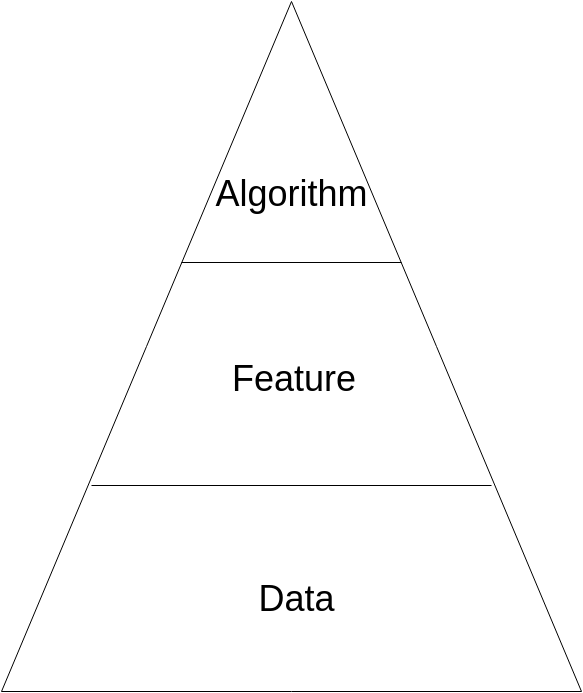
\includegraphics[scale=1.5]{data.png}
\caption{Importance of factors to the performance of ML application}
\label{fig:datai}
\end{figure}

However, in the age of big data \cite{lohr2012age}, large datasets are collected automatically so bias are inevitable among the datasets, therefore, unrealistic results will be obtained from training/testing dataset using the above \textit{experimental paradigm} \cite{torralba2011unbiased}. So for most current researches the models are trained and tested based on one single dataset, the classifiers learned can only work under a certain statistical distribution of the data. Only if with the updates of the model, can the classifiers trained from the old campaigns be applied to new campaigns in the concept of online advertisement. Therefore, under the situation that the advertising data from different advertiser campaigns behave differently and largely biased, according to the idea in \cite{threethings2015} and \cite{domingos2012few}, representation of the data will be essential for machine learning algorithms. More informative data extracted from the dataset, more improvement in performance of the algorithm can be obtained, since digging out the insights from the dataset means filtering out the redundant information which are irrelevant to the prediction task. Therefore, we will focus on the process of \textit{Feature Extraction} or \textit{Feature Engineering} to reach the goal that, 
\begin{itemize}
\item  the new feature space is low dimensional to avoid the \textit{curse of dimensionality} which will be common in the age of \textit{Big Data}
\item the new feature space is informative and the irrelevant data are got rid of, while the performance of prediction task is still comparable to that of traditional binary feature.
\item  the new feature space can help partly solve the \textit{cold start} problem to generalize the model among different campaigns.
\end{itemize}

In this paper we postulate the concept of \textit{Counting Feature} which is the first time, to satisfy the above three requirements. To shortly introduce counting feature, the counting feature of each \textit{field} in the meta ad data is composed of two parts, i.e., \textit{frequency feature} and \textit{average CTR feature}. Frequency feature represents the marginal distribution of the items in the field, and average CTR feature shows the conditional distribution of the clicks on the items in that field. For example, for the field of \textit{City} in meta data there are 500 different cities, if Beijing appears 100,000 times in the dataset with a total number of 1,000,000 impressions, which in total lead to 100 clicks from clients, Hong Kong appears 50,000 times, which also bring 100 clicks for the advertiser. Then in the concept of counting feature, there will be only two features generated from this field of \textit{city}, and the counting values are continuous such as Beijing with frequency counting value 0.1 and average CTR counting value 0.001, Hong Kong with frequency counting value 0.05 and average CTR counting value 0.002. But for binary feature which is encoded into one-hot feature, there will be 500 unique feature generated from the field \textit{city} with only one feature as 1 and others as 0 for each impression, which is sparse and redundant. The goal of low dimension feature space can be achieved by the construction of counting feature based on the statistical property of the dataset. 

What's more, admitting the existence of the bias in the dataset, we prove that the performance of counting feature using non-linear logistic regression model is comparable to that of binary feature using linear logistic regression model. Generally, binary features can be widely used in linear regression based estimators such as logistic regression. Counting features can be used in the tree models such as random forest or gradient boosting regression tree for their continuity property, and they can achieve similar performance in the two situations. To the best of our knowledge, there is no work extensively studying the comparison and relationship of these two kinds of features. Particularly,this is the first time that counting feature based CTR estimation is discussed.  

The classical \textit{Cold Start} problem for online learning is the biggest barrier to meet the 3rd requirement. In the scope of online advertising CTR prediction, cold start problem can be interprated that with the knowledge from old advertisement campaigns, how to apply them to new campaigns which are lack of information initially, in order to avoid repetitive work of data collection and model construction, to make sure that large-scale industry online implementation of CTR prediction system feasible. Most of the current research such as \cite{mohan2011web} \cite{chu2011unbiased} \cite{he2014practical} and \cite{mcmahan2013ad} regard it as an active learning problem, the parameters of the model are regarded as a probability distribution and with the help of Bayesian probit method, the parameters can be updated as new data comes in thus enhancing the precision of CTR prediction for new campaign. However, in the time of big data, online data stream is extremely huge which cost resources and time for the updating of the model. In our work, we try to build a general cross domain model which can be used for each advertisement campaign without the tedious process of model updating. Different from binary feature based model, in which the number of features is variable and feature value is fixed (0 and 1), counting feature benefits from the truth that its number of features is static and feature value can be variable, thus transforming the variability form weight space of the model to the feature space. The counting feature value for each item in each field can be updated with the increasing amount of statistical information gathered from the new campaign. We prove that counting feature performs significantly better than binary feature with high dimensions in terms of cross-domain CTR prediction, the experimental results also show that with the increasing volume of statistical information gathered from new campaign, AUC increases accordingly for counting feature model but with no impact on binary feature based model.

In summary, the contributions of this paper are as follows:
\begin{itemize}
\item We find the relation between binary feature and counting feature and show that their performances for CTR prediction are comparable under certain situation.
\item We research on cross domain learning problem and prove that cold start problem in the field of online advertising CTR prediction is in the scope of \textit{Domain Adaptation} problem. We also show the proofs that only domain distributions differ between old and new advertisement campaigns, the assumption of same task between two campaigns is convincing. 
\item We show that the performance of counting feature in cross domain learning problem for CTR prediction compared to binary feature and validate that counting feature's performance is significantly better than that of binary feature.
\end{itemize}
The rest of the paper is organised as follows, section 2 discusses the related work, our justification of counting feature is formulated in section 3 and in section 4 we discuss on the cross domain problem for online advertisement and model generalization, experiment results are shown in section 5 and we conclude in the last section.

%Inline citation: \bibentry{example-citation}

% This just dumps some pseudolatin in so you can see some text in place.


\chapter{Related Work}
\label{chapterlabel2}

\section{CTR Prediction}
Click-Through Rate (CTR) prediction is a well-studied online advertising problem in recent years. Advertisers tend to use CTR as a metric for the evaluation of the performance effectiveness of online advertising system to better predict their cost and revenue economically. CTR prediction is important for both sponsored search and RTB industry. 
Billions of dollars are being spent on sponsored advertising a year, predicting the possibility of the click for a specific ad in response to a certain query from the user is crucial to the business model of search engine industry. For sponsored search, in \cite{richardson2007predicting}, Microsoft tends to build a ML model making use of the features of ads, terms, and advertisers to predict the click probability for new ad, which can not only increase the revenue of the website, but also the user satisfactory. Logistic regression model is used to train the historical information of the ads and it is used to predict the CTR of new ad. It also shows that the position of the ad on the webpage largely decides the attraction of the ad. \cite{graepel2010web} shows an \textit{adPredictor} model to interpret the CTR as a linear combination of weighted features to realize a Bayesian online algorithm, the weights space is regarded as a Gaussian prior distribution and its mean and variance can be updated with the income of new data. \cite{zhu2010novel} proposes a General Click Model (GCM) upon a Bayesian network and \textit{Expectation Propagation} method is used to perform approximate Bayesian inference. It shows that all the other models are just the special cases of GCM. \cite{mcmahan2013ad} proposes a system which aims to train massive models on massive data with minimum resources, the linear model of logistic regression is used, but a new way of regularization which is similar to Regularized Stochastic Learning (RDA) is realized for gradient descent. This method is easier to implement and able to improve the final accuracy. As a trick, the method of probabilistic feature inclusion is used to select the features which can be used to avoid the long-tailed distribution of features, thus improving the accuracy of prediction and save the memory of machines meanwhile.

Besides sponsored search, many companies also set foot in RTB industry, Google provides a detailed and comprehensive report about the industry\cite{google2015}, since we are standing at the age of the intersection of data liquidity and inventory liquidity with the rise of exchangers and advertisers who have brought much more liquidity for the market, advertisements have a huge amount of ways to be presented to the potential audience, RTB is a revolutionary business model for display advertisement, as shown in Figure \ref{fig:ctr} the media buyers do not need to buy the advertising slots from millions of individual sites which is operationally impossible, but from a single DSP. A more efficient, faster and automated way is realized by RTB for advertisers to buy slots among sites more easily. 

Many researches in the field of RTB have been done. Besides the common linear model , non-linear model, such as tree based models and deep learning are all used for the CTR prediction in the context of RTB. In \cite{agarwal2010estimating} LMMH (Log-linear Model for Multiple Hierarchies) is proposed to solve the problem of estimating CTR for high dimensional and multivariate categorical data, the tree-like model is used in which the weight for each pair of node can be stored so that the click probability can be modelled as a product of the weights for all the pairs of nodes. \cite{trofimov2012using} proposes a boosting tree method which is a MatrixNet machine learning algorithm showing better performance than linear and logistic regression model. \cite{he2014practical} combines decision tree and logistic regression model together, the fundamental idea is to transform the original feature space into the \textit{right} feature space using boosting tree model, the right feature space can highly improve the CTR prediction performance in terms of AUC, instead of manually processing of feature selection and combination, boosting tree is able to generate the appropriate features which are the leafs of the tree. In order to keep the freshness of model, the model will be trained on a daily basis. It shows that the the combination of decision tree and logistic regression model can generate the right features, as well as using the right model, which will perform much better than selecting high value features and complex model.

\begin{figure}[h]
\centering
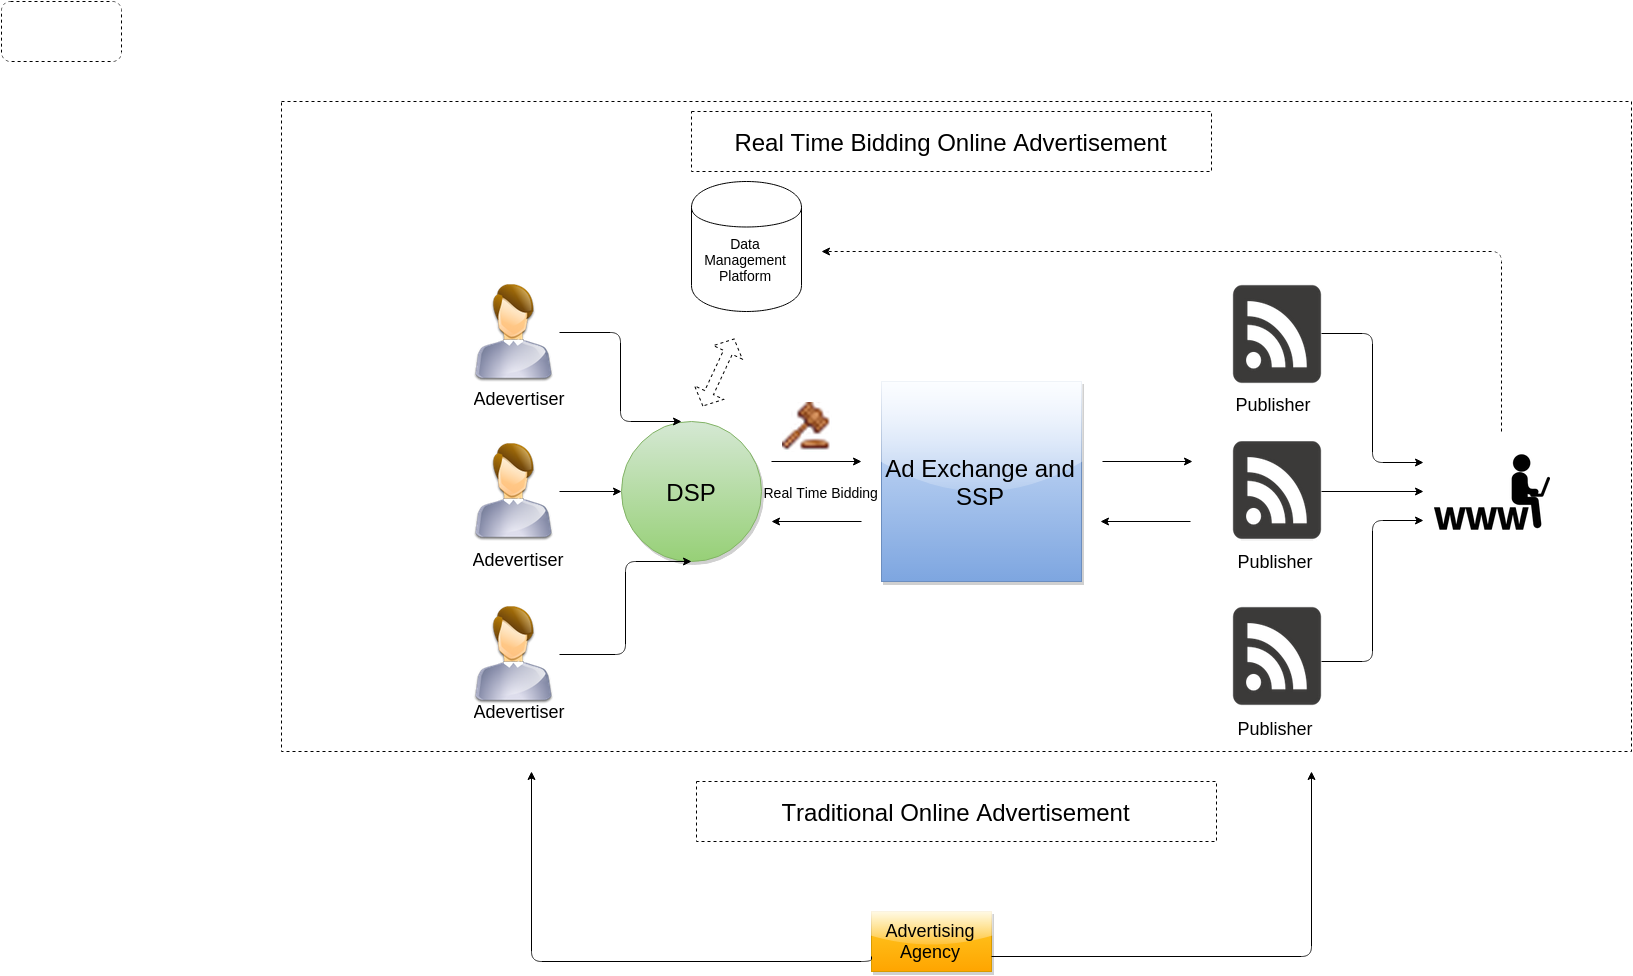
\includegraphics[width=\columnwidth]{rtblanscape.png}
\caption{Comparison between Real Time Bidding and Traditional Online Advertising}
\label{fig:ctr}
\end{figure}

\cite{cheng2012multimedia} conducts an experiment on over billions of impressions. There are also other researches on CTR prediction problem, \cite{richardson2007predicting} makes use of logistic regression to predict clicks. \cite{mcmahan2013ad} discusses on the practical engineering of CTR estimation as well as the performance of applying traditional machine learning model on complex huge dataset. \cite{zhu2010novel} discusses on General Click Model based on Bayesian network. \cite{graepel2010web} talks about \textit{Online Bayesian Probit Regression}. \cite{mohan2011web} discusses on the use of \textit{Gradient Boosting Regression Tree} (GBRT) on web ranking. GBRT algorithm is commonly used in the industry now, which is a non-linear classifier composed of a set of separators, by stacking a GBRT with LR to eliminate the non-linearity in the features it is able to give better CTR prediction results.

In conclusion, the researches on CTR are abundant for linear or non-linear regression model for sponsored search and RTB, namely how to find the \textit{right model}. However, in real industry, due to the unstructured and complex characteristic of the data, the pre-processing of data before putting into the model is more important for a real-world CTR prediction, the researches on \textit{Feature Engineering} is rare, and most of them is in the field of \textit{Natural Language Processing} (NLP), such as in \cite{garla2012ontology}, which makes use of the domain knowledge in biomedical to encode in the \textit{Unified Medical Language System} so that the machine learning clinical text classification performance can be improved largely. As said by Mohammad Pezeshki in \cite{featureengineering}

\textit{Actually the success of all Machine Learning algorithms depends on how you present the data.}

A good feature engineering means, the feature space is more flexible and easier, which means less complex model can be used but still obtain good performance, as the work in \cite{he2014practical}, the binary feature space is transformed into a lower dimension space using decision tree. Similar, in our paper, contrary to most of the researches in CTR prediction problem which focus on ML models, we will turn our focus on a more fundamental problem, namely how to prepare a better feature space for the model training.   

\section{Cold Start Problem}
The main purpose of this paper is to solve the cold start problem for CTR prediction, namely we use the data from old advertisement campaigns to predict the CTR in the new advertisement campaigns. Considering the complex and unpredictable of human behavior, this is a complicated problem. Few researches have been done to solve the cold start problem in the field of online advertising, therefore we will start to research on cold start problem in the area of \textit{recommendation system} with more abundant resources.

Cold start is a classical problem in the field of recommendation system, it focuses on the issues when the system is at the start stage without enough information so no inferences for users or items can be drew. \textit{Collaborative Filtering} (CF) is the most popular method proposed to solve this problem. In \cite{schein2002methods}, content and collaborative data are combined to solve the problem under a single probabilistic framework. \cite{su2009survey} provides a comprehensive review of collaborating filtering methods, model-based, memory-based and hybrid CF algorithms are discussed in this paper. There are also some papers focusing on solving the cold start problem based on the data itself. \cite{li2013news} proposes a personalized news recommendation model to apply ranking on hypergraph that includes users, news articles, and topics. The motivation that the researcher apply the hypergraph in news personalized recommendation is that for a news recommendation system, mining implicit relations among users, news articles, topics and named reading community is important. Given the special properties of the news articles, the researchers partition the hypergraph into multiple fine-grained 
ones, and then transform the recommendation problem into a ranking problem among the fine-grained hypergraphs. After that, the similarity graph of the news articles are built, namely setting the weights of the hyperedge. Finally, the transductive inference is performed on the news capsule in order to derive the news based on the user’s preference to provide the recommendation list for the user. \cite{jiang2012social} addresses the problem of sparsity and cold start in social recommendation. The researchers propose a \textit{Hybrid Random Walk} (HRW) algorithm to integrate multiple heterogeneous domains using signed/unsigned links,directed/undirected links and within-domain/cross-domain links into a star-structured hybrid graph in which user graph is at the center. A random walk is performed until its convergence and the steady state distribution is used for recommendation. \cite{feng2012incorporating} proposes a supervised random walk for setting of personalized tag recommendation. In this article, the heterogeneous information in the social tagging system, such as users’ tagging behaviors, tag semantics, social networks and item profiles are implemented to help alleviate the cold start problem due to data sparsity.

The above researches all focus on recommending novel items to the users based on information from heterogeneous information sources, they are not directly related to CTR prediction directly since the authors all regard data as vertex and use edge to represent the relations between the data, but we can get the insights from the literature that the information from old domains can be somewhat transformed to the new domain for the recommendation of new item. Since we can regard CTR prediction problem as a typical recommendation problem, in which advertisements with higher probability to be clicked will be recommended to the users. Therefore based on the information from the user, the advertisement itself, and the context information, we can find the position of the user profile in the network organized by these information, which confirms the certain level of generalization of the data distribution among all the domains. Therefore, it is possible to predict the CTR for new users based on the historical data as long as the logical relations exist between the historical data and the new user. 

The only paper focusing on cold start problem in the field of online advertising is \cite{agarwal2009regression}, which proposes a \textit{Regression Latent Factor} to incorporate entity features into latent factor learning. In this way the historical data and new item data can be combined together to improve the generalization of the model. We can conclude that getting the comprehensive information from history and to some point make use the new information will be a feasible way to solve the cold start problem for CTR prediction.

\section{Domain Adaptation}
In order to solve the cold start problem, we need to make use the old information in history. In the aspect of online advertising, it means how to transform the knowledge from source domains, namely old campaigns to the target domain, which is the new campaign.

The concept of domain adaptation is derived from \textit{Transfer Learning}, transfer learning is a popular research topic in the fields of artificial intelligence, machine learning, NLP, etc. In the field of machine learning, different from traditional predictive machine learning methods which ignore the difference between training and test datasets, in real world, the source and target sets should suffer from the situation of \textit{dataset shift} \cite{quionero2009dataset}, therefore, transfer learning will play a role to transfer the knowledge from current advertisement campaigns to the new ones. 

\cite{pan2010survey} makes a detailed discussion on transfer learning focusing on categorizing transfer learning for regression, classification and clustering problems. When the source and target tasks are different, and the source and target domains are same, it is called \textit{inductive transfer learning}, when the source and target domains are different however the source and target tasks are the same, it is called \textit{transductive transfer learning}. The final goal of the transfer learning system is to equip the system with the ability to recognize and apply the knowledge learned in previous domains to novel ones, which share some point of commonality. \cite{dai2007transferring} proposes a method to solve the problem of transfer learning in text classification using an EM-based naive Bayes classifier, the initial probability distribution of the source domain is estimated and then the EM algorithm is used to revise the trained model for the test dataset distribution using the unlabeled instances, this research with \cite{jiang2007instance}, \cite{huang2006correcting} and \cite{bickel2007discriminative} can be regarded as the \textit{instance based approach}. The assumption of this approach is that the source and target domains own many overlapping features, the items in the source domain will be regarded as the samples from the target domain, and part of the labeled data in the source domain can be reused in the target domain after re-weighting, the a rejection process will be made and the samples will be re-weighted again to map the target domain to the source domain to make the distributions similar. In this way, an adaptive feature representation should be developed to overcome the difference between the source and target domains. 

Another approach is \textit{feature representation transfer}, such as the researches in \cite{dai2007co}, \cite{ando2005high}, and \cite{blitzer2006domain}. In \cite{dai2007co}, a co-clustering algorithm is proposed to classify out-of-domain documents, the class label information given by the source domain can be extracted to label the word clusters for target domain. In \cite{blitzer2006domain} the domain adaptation problem in sentiment classification is discussed. No labeled data for the new domain is needed, at first \textit{N} pivot features are identified, then \textit{N} classifiers are built to predict the pivot features from remaining features, after that by computing the top eigenvectors the shared feature space can be discovered, and then the classifiers can be trained on the source domain using the augmented features. In brief, the approach of \textit{feature representation transfer} is based on the assumption that the source and target domains only share a part of the features, so the difference between the two domains can be solved by minimising the distances between the two domains, or using a multitask model to optimize the feature spaces of the two domains. In \cite{pan2011domain} the authors map the source and target domain data to the latent space spanned by the factors which can reduce domain difference and preserve original data structure. \cite{gao2008knowledge} is an example of the method \textit{parameter transfer}, which aims to discover the shared parameters or priors between the source and target domains. This approach is based on the assumption that the marginal distribution of feature space for target-domain and source-domain are similar, and also conditional probabilities also ought to be similar. In this way the parameter learned from the source domain can benefit the model for target domain. 

Our focus of this paper is to make use of transfer learning for CTR prediction problem of new advertisement campaigns. For the CTR problem, it is reasonable to say tasks between old and new campaigns are the same, which is a binary prediction classifier, however, the domains of the two will be distinct due to different data distribution and feature sets. 

From the above literature, we can make the following conclusions that we can refer to for our research. Firstly, the feature spaces of the source and target domains should be somewhat related, only if then can we transfer the knowledge learned from the source domain to the target domain, this is reasonable for the CTR problem, since even though the feature distribution from the old advertisement campaign and the new campaign can be different, the human behaviors should be related, namely the advertisements which can induce people to click should have some commonality. Secondly, the knowledge of the feature space and parameters from the model from the source domain can both benefit the CTR prediction model training in target domain. 

We also borrow the concept of \textit{domain shift} during our experiment, the comprehensive introduction of domain shift can be shown in the book \cite{quionero2009dataset}. The domain shift happens when the distribution of dataset changes arbitrarily, so the training data cannot be used directly to make predictions on the test domain. In this paper we will focus on \textit{covariate shift}, with the situation that \(Pr_{source}(x,y)\) and \(Pr_{target}(x,y)\) only differ in the marginal distribution of covariate \cite{zhang2013domain}, in the paper, we propose a machine learning method to quickly check whether the covariate shift exists between source and target datasets, ignited by the idea from \cite{coviriate}.






 











\chapter{Preliminaries}
\label{chapterlabel3}
\begin{table}[h]
\center
\vspace{-5pt}
\caption{Notations and descriptions.}
\label{tab:notation-des}
\small
\begin{tabular}{rl}
Notation & Description\\
\hline
\\ [-2.0ex]
$\bs{x_{\text{b}(N\times D)}}$ & The one-hot binary feature space.\\
$\bs{x_{\text{c}(N\times D)}}$ & The continuous counting feature space.\\
$\bs{y_{(1\times N)}}$ & The click result space\\
$w_{\text{b}(1\times D)}$ & The weights vector space of binary feature\\
$w_{\text{c}(1\times D)}$ & The weights vector space of counting feature\\
$T_{(M\times D)}$ & Transform Binary Feature to Counting Feature matrix\\
$A_{(N\times 1)}$ & Calculating frequency matrix which is an all-one vector $\vec{1 }$\\
$C_{(M\times D)}$ & Field  matrix which is a 0-1 matrix concatenated with \textsl{}{M} \\
& vectors \(V_{m,(m = 1...M)}\) and in each vector \(V_m\) only its \\
& corresponding positions in field \textsl{m} is filled with 1, \\
& with other positions 0. \\
$Diag$ & Transform the column vector into a diagonal matrix
\end{tabular}
\end{table}

\chapter{Conclusions and Future Work}
\label{conclusion}
In this project, we introduce the concept of \textit{counting feature} which is composed of \textit{frequency feature} and \textit{average CTR feature}, and prove that for the same dataset, counting feature space is a non-linear transformation of binary feature space, and the CTR prediction performance in terms of AUC of counting feature using GBRT algorithm is comparable to that of binary feature using linear logistic regression model. Unlike previous and current researches which focus more on the improvement of machine learning model and algorithm in CTR prediction problem, we turn to the more fundamental, but more crucial to the industry, research field, which is feature engineering. We show that counting feature can not only transform the extremely high dimension feature space into low, scalable, interpretable space, but also remain the comparable CTR prediction performance as traditional method, which will largely decrease the memory and time cost for industry. 

To the best of our knowledge, our work is the first one to systematically research on statistical feature, namely counting feature, even though statistical feature has been used by a small range of companies in daily business, our work is the first one to not only provide experimental result, but also mathematical derivation. The most important thing is, we present that counting feature can partly solve the classical \textit{cold start} problem to extend the knowledge from one advertising campaign to the others, we show that without updating old model parameters we can still obtain high performance using counting feature in the context of \textit{cross-domain learning} problem. There are few literature studying on cross-domain learning problem in the field of online advertising, and we are the first one with simplest implementation and solid backups.

However, the research in of our work is not ended. Firstly, we need more dataset to test our theory since currently we only have two datasets which are from iPinYou and Adform, also more linear and non-linear machine learning algorithms should be used to validate the correctness of our theory. Secondly, now we can only do the offline experiment, however, since for cross-learning problem, commonly the new income data should be in the format of stream, we already mimic the process of data stream, but implementing the experiment online will be absolutely what we will do next. Lastly, for the cross-learning problem, now we assume that the marginal distribution of the joint probability distribution of feature and label space are the same so that directly using model from old campaign to new ones is feasible, however, the covariate or domain shift is inevitable in the real world machine learning problem, a multitask optimization method to not only minimise the different between the feature distribution of source and target campaign, but also classifier difference should be studied to increase the CTR prediction further.

%\addcontentsline{toc}{chapter}{Appendices}

% The \appendix command resets the chapter counter, and changes the chapter numbering scheme to capital letters.
%\chapter{Appendices}
\appendix
\chapter{List of Code}
\label{appendixlabel1}
1. Make Feature \\
(1). Make Binary Feature
\lstset{language=Python, 
        basicstyle=\ttfamily\small, 
        keywordstyle=\color{blue},
        commentstyle=\color{comments},
        stringstyle=\color{black},
        showstringspaces=false,
        identifierstyle=\color{black}}
\begin{lstlisting}[numbers=left, breaklines=true]
import pandas as pd
import sys
import numpy as np
import operator
import random
from collections import Counter
from math import sqrt
from random import shuffle
import math
def getsecondfeature(frame_train_count):
    columns1= ['log_date', 'log_time_hour', 'client_id', 'placement_id', \\
    'inventory_source_id', 'url', 'position_id', 'size', 'browser_id', \\
'os_id', 'user_agent', 'screen_size_id', 'visited_domains', 'visited_logpoints', 'clicker']
    count_valid = {}
    second = {}
    second_valid = {}
    second_whole = []

    for idx1, val1 in enumerate(columns1):
        for idx2, val2 in enumerate(columns1[idx1+1:]):
            second[val1] = frame_train_count.groupby([val1, val2])\\
            [val1].count()
            second_valid[val1] = [key for key in second[val1].keys() if \\
            second[val1][key] > 10000]
            second_whole.extend(second_valid[val1])
            second_whole.append(val1+':other')\\
    return second_whole

def notlast(itr):
    itr = iter(itr)  # ensure we have an iterator
    prev = itr.next()
    for item in itr:
        yield prev

        prev = item
print 'start'
file = sys.argv[1]
file = int(float(file))
cnt = Counter()
ctrcount = Counter()
pd.options.display.float_format = '{:.25f}'.format

columns = ['log_date', 'log_time_hour',
           'inventory_source_id', 'position_id', 'size', 'browser_id', 'os_id', 'user_agent',
           'screen_size_id', 'visited_domains', 'visited_logpoints', 'clicker', 'click_count']

columns1= ['log_date', 'log_time_hour', 'client_id', 'placement_id',
           'inventory_source_id', 'domain', 'url', 'position_id', 'size', 'browser_id', 'os_id', 'user_agent',
           'screen_size_id', 'visited_domains', 'visited_logpoints', 'clicker']

path_train_train = '%d/train.train.txt' % file
path_train_count = '%d/train.count.txt' %file
path_test_test = '%d/test.test.txt' % file
path_test_valid = '%d/test.valid.txt' % file

fo_train = open('%d/train.bi.txt' %file, 'w')
fo_test_test = open('%d/test.bi.test.txt' % file, 'w')
fo_test_valid = open('%d/test.bi.valid.txt' % file, 'w')
fo_index = open('%d/index.txt' % file, 'w')

frame_train_train = pd.read_csv(path_train_train,dtype=str,\\
error_bad_lines = False)
frame_train_count = pd.read_csv(path_train_count,dtype=str,\\
error_bad_lines = False)
frame_test_test = pd.read_csv(path_test_test,dtype=str,\\
error_bad_lines = False)
frame_test_valid = pd.read_csv(path_test_valid,dtype=str,\\
error_bad_lines = False)
total_length = len(frame_train_count)
dict_unique = {}

length = 0
frame_train_count = pd.DataFrame(frame_train_count, columns=columns)

for c_index in range(0, len(columns) - 1):
    seri_train_count = frame_train_count.ix[1:len(frame_train_count)-1,\\
    c_index]

    seri_train_count = seri_train_count[~seri_train_count.isnull()]
    unique_s = seri_train_count.unique()
    unique_s = unique_s.tolist() + ['other']
    index = 0
    unique_list = []
    dict_u = {}
    for u in range(0, len(unique_s)):
        dict_u[unique_s[u]] = u + length
    dict_unique[columns[c_index]] = dict_u
    length = length + len(unique_s)
index = 0
record_length = 0
for column in notlast(columns):
    index = index + 1
    dict_u = dict_unique[column]
    record_length = record_length + len(dict_u)
    for key in dict_u:
        fo_index.write(str(index) + ':' + str(key) + ' ' + str(dict_u[key]))
        fo_index.write('\n')
record_length = record_length + 100
record_length = 2155314

        # ctr[column] = (frame_train_ctr.groupby(column).size()/float(count[column])).fillna(0)
for index, row in frame_train_train.iterrows():
    if row[-1] == str(0) or row[-1] == 0:
        fo_train.write(str(0))
    else:
        fo_train.write(str(1))

    for column in notlast(columns):
        dict_u = dict_unique[column]
        if row[column] not in dict_u:
            id = dict_u['other']
            fo_train.write(' ' + str(id) + ':' + str(1))
        else:
            id = dict_u[row[column]]
            fo_train.write(' ' + str(id) + ':' + str(1))

    fo_train.write('\n')
fo_train.close()

for index, row in frame_test_test.iterrows():
    if row[-1] == str(0) or row[-1] == 0:
        fo_test_test.write(str(0))
    else:
        fo_test_test.write(str(1))

    for column in notlast(columns):
        dict_u = dict_unique[column]
        if row[column] not in dict_u:
            id = dict_u['other']
            fo_test_test.write(' ' + str(id) + ':' + str(1))
        else:
            id = dict_u[row[column]]
            fo_test_test.write(' ' + str(id) + ':' + str(1))

    fo_test_test.write('\n')
fo_test_test.close()

\end{lstlisting}
(2) Make Counting Feature
\lstset{language=Python, 
        basicstyle=\ttfamily\small, 
        keywordstyle=\color{blue},
        commentstyle=\color{comments},
        stringstyle=\color{black},
        showstringspaces=false,
        identifierstyle=\color{black}}
\begin{lstlisting}[numbers=left, breaklines=true]
import pandas as pd
import sys
import operator
import random
from collections import Counter
from math import sqrt
from random import shuffle
import math
import matplotlib.pyplot as plt
import numpy as np

def notlast(itr):
    itr = iter(itr)  # ensure we have an iterator
    prev = itr.next()
    for item in itr:
        yield prev
        prev = item
def median(mylist):
    sorts = sorted(mylist)
    length = len(sorts)
    if not length % 2:
        return (sorts[length / 2] + sorts[length / 2 - 1]) / 2.0
    return sorts[length / 2]

def k_means(data_pts, k=None):
    """ Helper functions """

    def lists_are_same(la, lb):  # see if two lists have the same elements
        out = False
        for item in la:
            if item not in lb:
                out = False
                break
            else:
                out = True
        return out

    def distance(a, b):  # distance between (x,y) points a and b
        return sqrt(abs(a[0] - b[0]) ** 2 + abs(a[1] - b[1]) ** 2)

    def average(a):  # return the average of a one-dimensional list (e.g., [1, 2, 3])
        return sum(a) / float(len(a))

    """ Set up some initial values """
    if k is None:  # if the user didn't supply a number of means to look for, try to estimate how many there are
        n = len(data_pts)  # number of points in the dataset
        k = int(sqrt(n / 2))  # number of clusters - see
        #   http://en.wikipedia.org/wiki/Determining_the_number_of_clusters_in_a_data_set#Rule_of_thumb
    if k < 1:  # make sure there's at least one cluster
        k = 1

    """ Randomly generate k clusters and determine the cluster centers,
        or directly generate k random points as cluster centers. """

    init_clusters = data_pts[:]  # put all of the data points into clusters
    shuffle(init_clusters)  # put the data points in random order
    init_clusters = init_clusters[0:k]  # only keep the first k random clusters

    old_clusters, new_clusters = {}, {}
    for item in init_clusters:
        old_clusters[item] = []  # every cluster has a list of points associated with it. Initially, it's 0

    while 1:  # just keep going forever, until our break condition is met
        tmp = {}
        for k in old_clusters:  # create an editable version of the old_clusters dictionary
            tmp[k] = []

        """ Associate each point with the closest cluster center. """
        for point in data_pts:  # for each (x,y) data point
            min_clust = None
            min_dist = 1000000000  # absurdly large, should be larger than the maximum distance for most data sets
            for pc in tmp:  # for every possible closest cluster
                pc_dist = distance(point, pc)
                if pc_dist < min_dist:  # if this cluster is the closest, have it be the closest (duh)
                    min_dist = pc_dist
                    min_clust = pc
            tmp[min_clust].append(point)  # add each point to its closest cluster's list of associated points

        """ Recompute the new cluster centers. """
        for k in tmp:
            associated = tmp[k]
            xs = [pt[0] for pt in associated]  # build up a list of x's
            ys = [pt[1] for pt in associated]  # build up a list of y's
            x = average(xs)  # x coordinate of new cluster
            y = average(ys)  # y coordinate of new cluster
            new_clusters[(
            x, y)] = associated  # these are the points the center was built off of, they're *probably* still associated

        if lists_are_same(old_clusters.keys(), new_clusters.keys()):  # if we've reached equilibrium, return the points
            return old_clusters.keys()
        else:  # otherwise, we'll go another round. let old_clusters = new_clusters, and clear new_clusters.
            old_clusters = new_clusters
            new_clusters = {}

file = sys.argv[1]
file = int(float(file))
cnt = Counter()
ctrcount = Counter()
count = {}
ctr = {}
test_count = {}
pd.options.display.float_format = '{:.25f}'.format

columns = ['log_date', 'log_time_hour',
           'inventory_source_id', 'position_id', 'size', 'browser_id', 'os_id', 'user_agent',
           'screen_size_id', 'visited_domains', 'visited_logpoints', 'clicker', 'click_count']

path_train_train = '%d/train.train.txt' % file
path_train_count = '%d/train.count.txt' % file
path_test_test = '%d/test.test.txt' % file
path_test_valid = '%d/test.valid.txt' % file

fo_train = open('%d/train.countfeature.txt' % file, 'w')
fo_test_test = open('%d/test.countfeature.test.txt' % file, 'w')
fo_test_valid = open('%d/test.countfeature.valid.txt' % file, 'w')
fo_index = open('%d/index_count.txt' % file, 'w')
fo_count_index = open('%d/index_countfeature.txt' % file, 'w')

index = 0
for column in notlast(columns):

    fo_count_index.write(column + ':' + 'frequency' + ' ' + str(index))
    index = index + 1
    fo_count_index.write('\n')
    fo_count_index.write(column + ':' + 'averagectr' + ' ' + str(index))
    index = index + 1
    fo_count_index.write('\n')

#print 'start'
frame_train_train = pd.read_csv(path_train_train, dtype=str,error_bad_lines = False)
frame_train_count = pd.read_csv(path_train_count, dtype=str,error_bad_lines = False)
frame_test_test = pd.read_csv(path_test_test, dtype=str,error_bad_lines = False)
frame_test_valid = pd.read_csv(path_test_valid, dtype=str,error_bad_lines = False)
total_length = len(frame_train_count)
test_total_length = len(frame_test_test)

for column in columns:
    count[column] = frame_train_count.groupby(column).size()
    test_count[column] = frame_test_test.groupby(column).size()

frame_train_ctr = frame_train_count[(frame_train_count.click_count == str(1))]
aver_count = {}
aver_ctr = {}

index = 1
for column in notlast(columns):
    count[column] = count[column].astype(float)
    #ctr[column] = math.log10((frame_train_ctr.groupby(column).size() / count[column]).fillna(0) + math.pow(10, -100))
    ctr[column] = ((frame_train_ctr.groupby(column).size() / count[column]).fillna(0))

    test_count[column] = test_count[column].astype(float)/float(test_total_length)
    count[column] = count[column].astype(float)/float(total_length)

    l = count[column].values.tolist()
    lctr = ctr[column].values.tolist()
    if len(l) == 0:
        aver_count[column] = 0

    else:
        aver_count[column] = sum(l)/float(len(l))
    if len(lctr) == 0:
        aver_ctr[column] = 0

    else:
        aver_ctr[column] = sum(lctr)/float(len(lctr))
        
# ctr[column] = (frame_train_ctr.groupby(column).size()/float(count[column])).fillna(0)
for index, row in frame_train_train.iterrows():
    id = 0
    if row[-1] == str(0) or row[-1] == 0:
        fo_train.write(str(0))
    else:
        fo_train.write(str(1))

    for column in notlast(columns):

        if column != 'click_count':

            if row[column] in count[column]:
                fo_train.write(' ' + str(id) + ':' + str(count[column][row[column]]))
                id = id + 1
                fo_train.write(' ' + str(id) + ':' + str(ctr[column][row[column]]))
                id = id + 1
            else:


                fo_train.write(' ' + str(id) + ':' + str(aver_count[column]))
                id = id + 1
                fo_train.write(' ' + str(id) + ':' + str(aver_ctr[column]))
                id = id + 1
    fo_train.write('\n')

fo_train.close()

for index, row in frame_test_test.iterrows():

    id = 0
    if row[-1] == str(0) or row[-1] == 0:
        fo_test_test.write(str(0))
    else:
        fo_test_test.write(str(1))

    for column in notlast(columns):

        if column != 'click_count':

            if row[column] in count[column]:

                fo_test_test.write(' ' + str(id) + ':' + str(count[column][row[column]]))
                id = id + 1
                fo_test_test.write(' ' + str(id) + ':' + str(ctr[column][row[column]]))
                id = id + 1
            else:
                fo_test_test.write(' ' + str(id) + ':' + str(aver_count[column]))
                id = id + 1
                fo_test_test.write(' ' + str(id) + ':' + str(aver_ctr[column]))
                id = id + 1
    fo_test_test.write('\n')

fo_test_test.close() 
\end{lstlisting}
2 Cold Start Experiment for Binary Feature
\lstset{language=Python, 
        basicstyle=\ttfamily\small, 
        keywordstyle=\color{blue},
        commentstyle=\color{comments},
        stringstyle=\color{black},
        showstringspaces=false,
        identifierstyle=\color{black}}
\begin{lstlisting}[numbers=left, breaklines=true]
import pandas as pd
import sys
import operator
import random
from collections import Counter
from math import sqrt
import math
import matplotlib.pyplot as plt
import collections
from random import shuffle
import subprocess
import os
import numpy as np


def log_10_product(x, pos):
    """The two args are the value and tick position.
    Label ticks with the product of the exponentiation"""
    return '%1i' % (x)


def k_means(data_pts, k=None):
    """ Helper functions """

    def lists_are_same(la, lb):  # see if two lists have the same elements
        out = False
        for item in la:
            if item not in lb:
                out = False
                break
            else:
                out = True
        return out

    def distance(a, b):  # distance between (x,y) points a and b
        return sqrt(abs(a[0] - b[0]) ** 2 + abs(a[1] - b[1]) ** 2)

    def average(a):  # return the average of a one-dimensional list (e.g., [1, 2, 3])
        return sum(a) / float(len(a))

    """ Set up some initial values """
    if k is None:  # if the user didn't supply a number of means to look for, try to estimate how many there are
        n = len(data_pts)  # number of points in the dataset
        k = int(sqrt(n / 2))  # number of clusters - see
        #   http://en.wikipedia.org/wiki/Determining_the_number_of_clusters_in_a_data_set#Rule_of_thumb
    if k < 1:  # make sure there's at least one cluster
        k = 1

    """ Randomly generate k clusters and determine the cluster centers,
        or directly generate k random points as cluster centers. """

    init_clusters = data_pts[:]  # put all of the data points into clusters
    shuffle(init_clusters)  # put the data points in random order
    init_clusters = init_clusters[0:k]  # only keep the first k random clusters

    old_clusters, new_clusters = {}, {}
    for item in init_clusters:
        old_clusters[item] = []  # every cluster has a list of points associated with it. Initially, it's 0

    while 1:  # just keep going forever, until our break condition is met
        tmp = {}
        for k in old_clusters:  # create an editable version of the old_clusters dictionary
            tmp[k] = []

        """ Associate each point with the closest cluster center. """
        for point in data_pts:  # for each (x,y) data point
            min_clust = None
            min_dist = 1000000000  # absurdly large, should be larger than the maximum distance for most data sets
            for pc in tmp:  # for every possible closest cluster
                pc_dist = distance(point, pc)
                if pc_dist < min_dist:  # if this cluster is the closest, have it be the closest (duh)
                    min_dist = pc_dist
                    min_clust = pc
            tmp[min_clust].append(point)  # add each point to its closest cluster's list of associated points

        """ Recompute the new cluster centers. """
        for k in tmp:
            associated = tmp[k]
            xs = [pt[0] for pt in associated]  # build up a list of x's
            ys = [pt[1] for pt in associated]  # build up a list of y's
            x = average(xs)  # x coordinate of new cluster
            y = average(ys)  # y coordinate of new cluster
            new_clusters[(
                x,
                y)] = associated  # these are the points the center was built off of, they're *probably* still associated

        if lists_are_same(old_clusters.keys(), new_clusters.keys()):  # if we've reached equilibrium, return the points
            return old_clusters.keys()
        else:  # otherwise, we'll go another round. let old_clusters = new_clusters, and clear new_clusters.
            old_clusters = new_clusters
            new_clusters = {}


def getplacement(path_train):
    frame_train = pd.read_csv(path_train)
    count = {}
    ctr = {}
    length = len(frame_train)
    frame_train_count = frame_train
    # print frame_train[:10]
    column = 'placement_id'

    count[column] = frame_train_count.groupby(column).size()
    count[column] = count[column].astype(float)
    frame_train_ctr = frame_train_count[(frame_train_count.click_count == 1)]
    ctr[column] = frame_train_ctr.groupby(column).size()
    dict_count = count[column]
    dict_ctr = ctr[column]
    clickhuge = [k for k in dict_ctr.keys() if dict_ctr[k] >= 500 and dict_count[k] >= 30000]

    return (count, ctr, clickhuge)

def getclient(path_train):
    frame_train = pd.read_csv(path_train)
    count = {}
    ctr = {}
    length = len(frame_train)
    frame_train_count = frame_train
    # print frame_train[:10]
    column = 'client_id'

    count[column] = frame_train_count.groupby(column).size()
    count[column] = count[column].astype(float)
    frame_train_ctr = frame_train_count[(frame_train_count.click_count == 1)]
    ctr[column] = frame_train_ctr.groupby(column).size()
    dict_count = count[column]
    dict_ctr = ctr[column]
    clickhuge = [k for k in dict_ctr.keys() if dict_ctr[k] >= 400]
    return (count, ctr, clickhuge)


cnt = Counter()
ctrcount = Counter()
pd.options.display.float_format = '{:.30f}'.format
file = sys.argv[1]
file = int(float(file))

path_train = '%d/train.log.txt' % file
path_test = '%d/test.log.txt' % file

ccc1 = []
ccc2 = []

cc1 = []
cc2 = []
c1 = sys.argv[2]
c1 = int(float(c1))
cc1.append(c1)
c2 = sys.argv[3]
c2 = int(float(c2))
cc2.append(c2)
column = 'client_id'
frame_train = pd.read_csv(path_train)
frame_test = frame_train

ccc1 = cc1
frame_train_wihout_cc = frame_train.loc[frame_train[column].isin(ccc1)]
rows = random.sample(frame_train_wihout_cc.index, (len(frame_train_wihout_cc.index) / 3))
frame_train_train = frame_train_wihout_cc.ix[rows]
frame_train_count = frame_train_wihout_cc.drop(rows)
print 'step1'
#ccc2.append(cc2[1])
ccc2 = cc2
frame_test_with_cc = frame_train.loc[frame_train[column].isin(ccc2)]
frame_test_with_cc=frame_test_with_cc.iloc[np.random.permutation(len(frame_test_with_cc))]
frame_test_with_cc = frame_test_with_cc.reset_index(drop=True)

wholelength = len(frame_test_with_cc)
print wholelength
windowrange = 50000

frame_test_test = pd.DataFrame()
frame_test_test_update = pd.DataFrame()
pace = 0

fo_result = open('%d/performance_ten_bi_%d_%d.txt' % (file,c1,c2), 'w')
print len(frame_test_with_cc)
    
print len(frame_train_train)
result = []
while (pace < wholelength - windowrange):
    new_data = frame_test_with_cc[pace:pace + windowrange - 1]
    
    if pace == 0:
        frame_train_train = [frame_train_train,frame_test_test[:windowrange/3]]
        frame_train_train = pd.concat(frame_train_train)
        frame_train_count = [frame_train_count,frame_test_test[(windowrange/3)+1:]]
        frame_train_count = pd.concat(frame_train_count)
        frame_test_test = new_data
        fo_train_train = open('%d/train.train.txt' % file, 'w')
        fo_train_count = open('%d/train.count.txt' % file, 'w')
        fo_test = open('%d/test.test.txt' % file, 'w')
        fo_test1 = open('%d/test.valid.txt' % file, 'w')

        frame_train_train.to_csv(fo_train_train, index=False)
        frame_train_count.to_csv(fo_train_count, index=False)
        frame_test_test.to_csv(fo_test, index=False)
        frame_test_test.to_csv(fo_test1, index=False)
        print pace/10000
        os.system("python -W ignore make_bi_new.py 11")
        rc = subprocess.Popen(['bash','/home/gaoxinyang/data/ctr-counting-features/models/lr/lr-driver.sh'],stdout=subprocess.PIPE)
        out = rc.communicate()[0]
        fo_result.write(out)
        fo_result.write('end')
    else:
    
        frame_test_test = new_data        
        #fo_train_count = open('%d/train.count.txt' % file, 'w')
        fo_test = open('%d/test.test.txt' % file, 'w')
        fo_test1 = open('%d/test.valid.txt' % file, 'w')

        frame_test_test.to_csv(fo_test, index=False)
        frame_test_test.to_csv(fo_test1, index=False)
        print pace/10000
        os.system("python -W ignore make_bi_new_update.py 11")
        #os.system("bash /home/gaoxinyang/data/ctr-counting-features/models/lr/lr-driver_update.sh")
        rc = subprocess.Popen(['bash','/home/gaoxinyang/data/ctr-counting-features/models/lr/lr-driver_update.sh'],stdout=subprocess.PIPE)
        out = rc.communicate()[0]
        fo_result.write(out)
        fo_result.write('end')
    pace = pace + windowrange
\end{lstlisting}
3. Cold Start for Counting Feature
\lstset{language=Python, 
        basicstyle=\ttfamily\small, 
        keywordstyle=\color{blue},
        commentstyle=\color{comments},
        stringstyle=\color{black},
        showstringspaces=false,
        identifierstyle=\color{black}}
\begin{lstlisting}[numbers=left, breaklines=true]
__author__ = 'gaoxinyang'
# !/usr/bin/python
__author__ = 'gaoxinyang'
import pandas as pd
import sys
import operator
import random
from collections import Counter
from math import sqrt
import math
import matplotlib.pyplot as plt
import collections
from random import shuffle
import subprocess
import os
import numpy as np


def log_10_product(x, pos):
    """The two args are the value and tick position.
    Label ticks with the product of the exponentiation"""
    return '%1i' % (x)


def k_means(data_pts, k=None):
    """ Helper functions """

    def lists_are_same(la, lb):  # see if two lists have the same elements
        out = False
        for item in la:
            if item not in lb:
                out = False
                break
            else:
                out = True
        return out

    def distance(a, b):  # distance between (x,y) points a and b
        return sqrt(abs(a[0] - b[0]) ** 2 + abs(a[1] - b[1]) ** 2)

    def average(a):  # return the average of a one-dimensional list (e.g., [1, 2, 3])
        return sum(a) / float(len(a))

    """ Set up some initial values """
    if k is None:  # if the user didn't supply a number of means to look for, try to estimate how many there are
        n = len(data_pts)  # number of points in the dataset
        k = int(sqrt(n / 2))  # number of clusters - see
        #   http://en.wikipedia.org/wiki/Determining_the_number_of_clusters_in_a_data_set#Rule_of_thumb
    if k < 1:  # make sure there's at least one cluster
        k = 1

    """ Randomly generate k clusters and determine the cluster centers,
        or directly generate k random points as cluster centers. """

    init_clusters = data_pts[:]  # put all of the data points into clusters
    shuffle(init_clusters)  # put the data points in random order
    init_clusters = init_clusters[0:k]  # only keep the first k random clusters

    old_clusters, new_clusters = {}, {}
    for item in init_clusters:
        old_clusters[item] = []  # every cluster has a list of points associated with it. Initially, it's 0

    while 1:  # just keep going forever, until our break condition is met
        tmp = {}
        for k in old_clusters:  # create an editable version of the old_clusters dictionary
            tmp[k] = []

        """ Associate each point with the closest cluster center. """
        for point in data_pts:  # for each (x,y) data point
            min_clust = None
            min_dist = 1000000000  # absurdly large, should be larger than the maximum distance for most data sets
            for pc in tmp:  # for every possible closest cluster
                pc_dist = distance(point, pc)
                if pc_dist < min_dist:  # if this cluster is the closest, have it be the closest (duh)
                    min_dist = pc_dist
                    min_clust = pc
            tmp[min_clust].append(point)  # add each point to its closest cluster's list of associated points

        """ Recompute the new cluster centers. """
        for k in tmp:
            associated = tmp[k]
            xs = [pt[0] for pt in associated]  # build up a list of x's
            ys = [pt[1] for pt in associated]  # build up a list of y's
            x = average(xs)  # x coordinate of new cluster
            y = average(ys)  # y coordinate of new cluster
            new_clusters[(
                x,
                y)] = associated  # these are the points the center was built off of, they're *probably* still associated

        if lists_are_same(old_clusters.keys(), new_clusters.keys()):  # if we've reached equilibrium, return the points
            return old_clusters.keys()
        else:  # otherwise, we'll go another round. let old_clusters = new_clusters, and clear new_clusters.
            old_clusters = new_clusters
            new_clusters = {}


def getplacement(path_train):
    frame_train = pd.read_csv(path_train)
    count = {}
    ctr = {}
    length = len(frame_train)
    frame_train_count = frame_train
    # print frame_train[:10]
    column = 'placement_id'

    count[column] = frame_train_count.groupby(column).size()
    count[column] = count[column].astype(float)
    frame_train_ctr = frame_train_count[(frame_train_count.click_count == 1)]
    ctr[column] = frame_train_ctr.groupby(column).size()
    dict_count = count[column]
    dict_ctr = ctr[column]
    clickhuge = [k for k in dict_ctr.keys() if dict_ctr[k] >= 500 and dict_count[k] >= 30000]

    return (count, ctr, clickhuge)

def getclient(path_train):
    frame_train = pd.read_csv(path_train)
    count = {}
    ctr = {}
    length = len(frame_train)
    frame_train_count = frame_train
    # print frame_train[:10]
    column = 'client_id'

    count[column] = frame_train_count.groupby(column).size()
    count[column] = count[column].astype(float)
    frame_train_ctr = frame_train_count[(frame_train_count.click_count == 1)]
    ctr[column] = frame_train_ctr.groupby(column).size()
    dict_count = count[column]
    dict_ctr = ctr[column]
    clickhuge = [k for k in dict_ctr.keys() if dict_ctr[k] >= 400]
    return (count, ctr, clickhuge)
cnt = Counter()
ctrcount = Counter()
pd.options.display.float_format = '{:.30f}'.format
file = sys.argv[1]
file = int(float(file))

path_train = '%d/train.log.txt' % file
path_test = '%d/test.log.txt' % file

# count_train, ctr_train, clickhuge_train = getplacement(path_train)

ccc1 = []
ccc2 = []
cc1 = []
c1 = sys.argv[2]
c1 = int(float(c1))
cc1.append(c1)

c2 = sys.argv[3]
c2 = int(float(c2))
cc2.append(c2)

ccc1 = cc1
frame_train_wihout_cc = frame_train.loc[frame_train[column].isin(ccc1)]
rows = random.sample(frame_train_wihout_cc.index, (len(frame_train_wihout_cc.index) / 3))
frame_train_train = frame_train_wihout_cc.ix[rows]
frame_train_count = frame_train_wihout_cc.drop(rows)
#ccc2.append(cc2[1])
ccc2 = cc2
frame_test_with_cc = frame_train.loc[frame_train[column].isin(ccc2)]
frame_test_with_cc=frame_test_with_cc.iloc[np.random.permutation(len(frame_test_with_cc))]
frame_test_with_cc = frame_test_with_cc.reset_index(drop=True)
#frame_test_with_cc = frame_test_with_cc.reindex(np.random.permutation(frame_test_with_cc.index))

wholelength = len(frame_test_with_cc)
#print wholelength
windowrange = 50000                          

frame_test_test = pd.DataFrame()
frame_test_test_update = pd.DataFrame()
pace = 0
fo_result = open('%d/performance_ten_count_%d_%d.txt' % (file,c1,c2), 'w')
result = []
while (pace < wholelength - windowrange):
    # if frame_test_with_cc.shape[0] > 150000: # len(df) > 10 would also work
    new_data = frame_test_with_cc[pace:pace + windowrange - 1]
    if pace == 0:
        frame_train_train = [frame_train_train,frame_test_test[:windowrange/3]]
        frame_train_train = pd.concat(frame_train_train)
        frame_train_count = [frame_train_count,frame_test_test[(windowrange/3)+1:]]
        frame_train_count = pd.concat(frame_train_count)

        frame_test_test = new_data
        fo_train_train = open('%d/train.train.txt' % file, 'w')
        fo_train_count = open('%d/train.count.txt' % file, 'w')
        fo_test = open('%d/test.test.txt' % file, 'w')
        fo_test1 = open('%d/test.valid.txt' % file, 'w')

        frame_train_train.to_csv(fo_train_train, index=False)
        frame_train_count.to_csv(fo_train_count, index=False)
        frame_test_test.to_csv(fo_test, index=False)
        frame_test_test.to_csv(fo_test1, index=False)
        os.system("python -W ignore make_count_new.py 11")
        #os.system("bash /home/gaoxinyang/data/ctr-counting-features/models/lr/lr-driver_count.sh")
        rc = subprocess.Popen(['bash','/home/gaoxinyang/data/ctr-counting-features/models/lr/lr-driver_count.sh'],stdout=subprocess.PIPE)

        out = rc.communicate()[0]
        fo_result.write(out)
        fo_result.write('end')
    else:
        
        frame_test_test_update = [frame_test_test_update,frame_test_test]
        frame_test_test_update  = pd.concat(frame_test_test_update)
        frame_test_test = new_data
        fo_train_count = open('%d/train.count.txt' % file, 'w')
        fo_test = open('%d/test.test.txt' % file, 'w')
        fo_test1 = open('%d/test.valid.txt' % file, 'w')
        frame_test_test_update.to_csv(fo_train_count, index=False)
        frame_test_test.to_csv(fo_test, index=False)
        frame_test_test.to_csv(fo_test1, index=False)
        
        os.system("python -W ignore make_count_new_update.py 11")
        #os.system("bash /home/gaoxinyang/data/ctr-counting-features/models/lr/lr-driver_count_update.sh")
        rc = subprocess.Popen(['bash','/home/gaoxinyang/data/ctr-counting-features/models/lr/lr-driver_count_update.sh'],stdout=subprocess.PIPE)
        out = rc.communicate()[0]
        fo_result.write(out)
        fo_result.write('end')
    pace = pace + windowrange
\end{lstlisting}
4. Marginal Distribution Generalization for Counting Feature (Similar to that of Binary Feature, and also for the generalization of feature space
\lstset{language=Python, 
        basicstyle=\ttfamily\small, 
        keywordstyle=\color{blue},
        commentstyle=\color{comments},
        stringstyle=\color{black},
        showstringspaces=false,
        identifierstyle=\color{black}}
\begin{lstlisting}[numbers=left, breaklines=true]
import datetime
import pprint

import numpy as np
import pandas as pd
from pandas.io.data import DataReader
import pylab as plt
import sklearn
from sklearn.cross_validation import train_test_split, KFold
from sklearn.linear_model import LinearRegression, LogisticRegression
from sklearn.metrics import mean_squared_error
from sklearn.pipeline import Pipeline
from sklearn.preprocessing import PolynomialFeatures
from sklearn.datasets import load_svmlight_file
from scipy import sparse

import pandas
import random
import math
from sklearn.metrics import roc_auc_score
from sklearn.metrics import confusion_matrix
from matplotlib import pyplot
from math import log
from collections import Counter
from sklearn.metrics import matthews_corrcoef


def sigmoid(p):
    p = max(p,-200)
    
    return 1.0 / (1.0 + math.exp(-p))

def pred(x,w_0,w):
    p = w_0
    
    for (feat, val) in x:
        
        if feat < 25:
          
          p += w[feat] * val 
    p = sigmoid(p)

    return p

def one_data_y_x(line,one_value):
    
    s = line.strip().replace(':', ' ').split(' ')

    
    y = int(s[0])
    x = []
    for i in range(1, len(s), 2):
        #val = 1
        if not one_value:
            
            try:
              val = float(s[i+1])
              #val = sigmoid(float(s[i+1])*weights[int(s[i])])
            except:
              val = 0
        x.append((int(s[i]), val))
    return (y, x)

def logistic_regression(one_v,feature_n,fi_train,fi_test,weights):
    np.random.seed(10)
    one_value = one_v
    k = 3
    learning_rate = 0.005
    weight_decay = 1E-30
    train_rounds = 10
    buffer_num = 1000000
    feature_index = {}
    index_feature = {}
    max_feature_index = 0
    feature_num = feature_n

    init_weight = 0.1
    w = np.zeros(feature_num)
    w_0 = 0

# train
    best_auc = 0.
    overfitting = False
    for round in range(1, train_rounds+1):
        
        #fi = open(sys.argv[1], 'r')
        line_num = 0
        train_data = []
        
        fi = open(fi_train, 'r')
        line_num = 0
        train_data = []
        while True:
            line = fi.readline().strip()
            
            if len(line) > 0:
                line_num = (line_num + 1) % buffer_num
                s = line.strip('\0').replace(':', ' ').split(' ')
                try:
                  train_data.append(one_data_y_x(line,one_value))
                except:
                  pass
                    
            if line_num == 0 or len(line) == 0:
                for data in train_data:
                    y = data[0]
                    x = data[1]
                # train one data
                    p = pred(x,w_0,w)
                    d = y - p
                    w_0 = w_0 * (1 - weight_decay) + learning_rate * d
                    for (feat, val) in x:
                        if feat < 25:
                            w[feat] = w[feat] * (1 - weight_decay) + learning_rate * d * val
                train_data = []
            if len(line) == 0:
                break
        fi.close()
        y = []
        yp = []
        fi = open(fi_test, 'r')
        for line in fi:
            s = line.strip('\0').replace(':', ' ').split(' ')
            if len(s) == 49:
              data = one_data_y_x(line,one_v)
              clk = data[0]
              pclk = pred(data[1],w_0,w)
              y.append(clk)
              yp.append(pclk)
        fi.close()
        ypp = map(lambda x: 1 if x > 0.5 else 0, yp)
        result = confusion_matrix(y,ypp)
        auc = roc_auc_score(y, yp)
        rmse = math.sqrt((mean_squared_error(y, yp)))
    
    return rmse
def create_lagged_series(symbol, start_date, end_date, lags=5):
    """
    This creates a pandas DataFrame that stores the percentage returns of the 
    adjusted closing value of a stock obtained from Yahoo Finance, along with 
    a number of lagged returns from the prior trading days (lags defaults to 5 days).
    Trading volume, as well as the Direction from the previous day, are also included.
    """

    # Obtain stock information from Yahoo Finance
    ts = DataReader(symbol, "yahoo", start_date-datetime.timedelta(days=365), end_date)

    # Create the new lagged DataFrame
    tslag = pd.DataFrame(index=ts.index)
    tslag["Today"] = ts["Adj Close"]
    tslag["Volume"] = ts["Volume"]

    # Create the shifted lag series of prior trading period close values
    for i in xrange(0,lags):
        tslag["Lag%s" % str(i+1)] = ts["Adj Close"].shift(i+1)

    # Create the returns DataFrame
    tsret = pd.DataFrame(index=tslag.index)
    tsret["Volume"] = tslag["Volume"]
    tsret["Today"] = tslag["Today"].pct_change()*100.0

    # If any of the values of percentage returns equal zero, set them to
    # a small number (stops issues with QDA model in scikit-learn)
    for i,x in enumerate(tsret["Today"]):
        if (abs(x) < 0.0001):
            tsret["Today"][i] = 0.0001

    for i in xrange(0,lags):
        tsret["Lag%s" % str(i+1)] = tslag["Lag%s" % str(i+1)].pct_change()*100.0

    tsret["Direction"] = np.sign(tsret["Today"])
    tsret = tsret[tsret.index >= start_date]
    return tsret
def validation_set_poly(random_seeds, degrees, X, y):
    """
    Use the train_test_split method to create a
    training set and a validation set (50% in each)
    using "random_seeds" separate random samplings over
    linear regression models of varying flexibility
    """
    sample_dict = dict([("seed_%s" % i,[]) for i in range(1, random_seeds+1)])
    
    for i in range(1, random_seeds+1):
        for d in range(1, degrees+1):
            polynomial_features = PolynomialFeatures(
                degree=d, include_bias=False
            )
            linear_regression = LogisticRegression()
            model = Pipeline([
                ("polynomial_features", polynomial_features),
                ("linear_regression", linear_regression)
            ])
            X_train, X_test, y_train, y_test = train_test_split(
                X, y, test_size=0.5, random_state=i
            )
            model.fit(X_train, y_train)
            # Calculate the test MSE and append to the
            # dictionary of all test curves
            y_pred = model.predict(X_test)
            
            test_mse = mean_squared_error(y_test, y_pred)
            print test_mse
            sample_dict["seed_%s" % i].append(test_mse)
           
    sample_dict["avg"] = np.zeros(degrees)
    for i in range(1, random_seeds+1):
        sample_dict["avg"] += sample_dict["seed_%s" % i]
    sample_dict["avg"] /= float(random_seeds)
    return sample_dict

def k_fold_cross_val_poly(folds, degrees,data,one_v,feature_n,weights):
    n = len(data)
    kf = KFold(n, n_folds=folds)
    kf_dict = dict([("fold_%s" % i,[]) for i in range(1, folds+1)])
    fold = 0
    for train_index, test_index in kf:
        fold += 1
        #print "Fold: %s" % fold
        data_train, data_test = data.ix[train_index], data.ix[test_index]
        fo_train = open('13/temp.train.txt' , 'w')
        fo_test = open('13/temp.test.txt' , 'w')
        data_train.to_csv(fo_train, index=False,sep=' ')
        data_test.to_csv(fo_test,index=False,sep=' ')
        fo_train_path = '13/temp.train.txt'
        fo_test_path = '13/temp.test.txt'
        for d in range(1, degrees+1):
            polynomial_features = PolynomialFeatures(
                degree=d, include_bias=False
            )
            
            test_mse = logistic_regression(one_v,feature_n,fo_train_path,fo_test_path,weights)

            kf_dict["fold_%s" % fold].append(test_mse)

    return kf_dict
if __name__ == "__main__":
    symbol = "^FTSE"

    index_file = [8908, 14501, 22134, 1414, 20224, 16280, 12482 ,1371, 15140, 20762]
    index_file1 = [8908, 14501, 22134, 1414, 20224, 16280, 12482 ,1371, 15140, 20762]
    
    result_variance = {}
    result_bi = []
    result_bi_mean = []
    result_bi_mean_auc = [] 
    result_bi_auc = []
    result_a_distance = []

    for index in range(0,len(index_file)):
    	#path = '13/train.bi.%d.txt' % index_file[index]
        path = '13/train.countfeature.%d.txt' % index_file[index]
        with open('/home/gaoxinyang/data/13/weights_count_%d.txt' %index_file[index]) as f:
        	lines = f.read().splitlines()
        	weights = lines
        	weights = [float(x) for x in weights] 
        data_train = pd.read_csv(path,dtype=str,error_bad_lines = False,header=None,sep = ' ')
        rows = random.sample(data_train.index, (len(data_train.index) / 200))
        data_train = data_train.ix[rows]
        data_train.ix[:,0] = int(1)
        print len(data_train)
        print index
        for index_test in range(0,len(index_file1)):
            print index_test
            path1 = '13/train.countfeature.%d.txt' % index_file1[index_test]
            data_test = pd.read_csv(path1,dtype=str,error_bad_lines = False,header=None,sep = ' ')
            #data_test = data_test[(data_test.ix[:,0] == str(1))]
            rows = random.sample(data_test.index, (len(data_test.index) / 200))
            data_test = data_test.ix[rows]
            
            data_test.ix[:,0] = int(0)
            print len(data_test)
            frames = [data_train,data_test]
            data = pd.concat(frames,ignore_index=True)
            data=data.iloc[np.random.permutation(len(data))]
            data = data.reset_index(drop=True)
    	    degrees = 1
    	    folds = 5
            kf_dict = k_fold_cross_val_poly(folds, degrees,data,False,24,weights)
    #print kf_dict
    	    rmse_ = []
            
    	    for fold in range(1,5):
        	x = kf_dict["fold_%s" % fold][0]
        	rmse_.append(x)
                    
            rmse_ = [x for x in rmse_ if x is not None]
            rmse_ = [x for x in rmse_ if x != 0]
    	    variance = np.std(rmse_)
            mean = np.mean(rmse_)
            a_distance = 2*(1-2*mean)
            result_bi_mean.append(mean) 
            result_bi.append(variance)
            result_a_distance.append(a_distance)
            result_bi_mean.append(mean) 
            result_bi.append(variance)
    fow = open('/home/gaoxinyang/data/13/result_count_variance.txt', 'w')
    for item in result_bi:
        fow.write("%s\n" % str(item)) 
    fow1 = open('/home/gaoxinyang/data/13/result_count_mean.txt', 'w')
    for item in result_bi_mean:
        fow1.write("%s\n" % str(item)) 
\end{lstlisting}









\lstset{language=Python, 
        basicstyle=\ttfamily\small, 
        keywordstyle=\color{blue},
        commentstyle=\color{comments},
        stringstyle=\color{black},
        showstringspaces=false,
        identifierstyle=\color{black}}
\begin{lstlisting}[numbers=left, breaklines=true]
\end{lstlisting}

 
% You could separate these out into different files if you have
%  particularly large appendices.

% This line manually adds the Bibliography to the table of contents.
% The fact that \include is the last thing before this ensures that it
% is on a clear page, and adding it like this means that it doesn't
% get a chapter or appendix number.
\addcontentsline{toc}{chapter}{Bibliography}

% Actually generates your bibliography.
\bibliography{example.bib}

% All done. \o/
\end{document}
